% Signé n'est pas sûr - article au format conférence IEEE (AI-ChainGuard, ESAIP Projet Applicatif 2). Version anglaise : signed_is_not_safe.tex
% Compilation :  cd paper && pdflatex signed_is_not_safe_fr.tex && pdflatex signed_is_not_safe_fr.tex   (babel-french requis ; présent sur Overleaf)
% Figures (variantes _fr) et chaque chiffre cité : python paper/figures/make_figures.py (lit results/, écrit figures/analysis.json)
\documentclass[conference]{IEEEtran}
\IEEEoverridecommandlockouts
\usepackage[utf8]{inputenc}
\usepackage[T1]{fontenc}
\usepackage[french]{babel}
\usepackage{cite}
\usepackage{amsmath,amssymb}
\usepackage{graphicx}
\usepackage{booktabs}
\usepackage{array}
\usepackage{xurl}
\usepackage{xcolor}
\usepackage{tikz}
\usetikzlibrary{arrows.meta,positioning,fit}
\usepackage{dblfloatfix}
\usepackage{flushend}
\usepackage[hidelinks]{hyperref}
\hypersetup{pdftitle={Signé n'est pas sûr : mesurer la frontière entre intégrité cryptographique et confiance sémantique dans les chaînes d'approvisionnement de l'IA},pdfauthor={Karan Deshmukh, Sudheer Reddy Jogi, Dola Krishna Dama, Rambabu Mekala},pdfsubject={ESAIP MSc Cybersécurité et Science des données, Projet Applicatif 2}}
\newcommand{\sys}{AI-ChainGuard}
\newcommand{\st}[1]{\textsc{#1}}
\newcommand{\role}[1]{{\fontsize{4.6}{5.2}\selectfont\ttfamily #1}}
\hyphenation{Signing Sigstore}
\addto\captionsfrench{\renewcommand{\tablename}{Tableau}\renewcommand{\figurename}{Fig.}\renewcommand{\abstractname}{R\'esum\'e}}
\renewcommand{\IEEEkeywordsname}{Mots-cl\'es}
\frenchsetup{StandardItemLabels=true,StandardLists=true,og=«,fg=»}

\begin{document}

\title{Signé n'est pas sûr : mesurer la frontière entre intégrité cryptographique et confiance sémantique dans les chaînes d'approvisionnement de l'IA}

\author{
\IEEEauthorblockN{Karan Deshmukh, Sudheer Reddy Jogi, Dola Krishna Dama, Rambabu Mekala}
\IEEEauthorblockA{MSc Cybersécurité et Science des données, ESAIP École d'Ingénieurs, Angers, France\\
Projet Applicatif 2 (projets d'IA appliquée), encadré par Sofiane Hamrioui\\
Auteur correspondant : domail2karandeshmukh@gmail.com}
}

\maketitle

\begin{abstract}
Un modèle déployé est le produit de jeux de données, de poids pré-entraînés et d'affinages venant de parties différentes ; or les contrôles de chaîne d'approvisionnement logicielle signent une compilation ou un fichier sans rien dire de cette filiation ni du sens d'une signature valide pour le comportement du modèle. Nous présentons \sys, qui donne à chaque artefact d'un pipeline d'IA, du jeu de données à l'enregistrement de déploiement, un manifeste signé contenant les empreintes des manifestes de ses parents : un graphe de provenance chaîné par hachage, soumis à dix contrôles, avec confiance et révocation dans un journal signé, ancré et en ajout seul, et une passerelle qui vérifie toute la chaîne au déploiement avant de charger le modèle. Nous \emph{mesurons} ensuite la frontière de ces garanties sur 48 variantes (attaques et témoins) en sept expériences. Toute manipulation de la suite postérieure à la signature, d'un poids modifié de $10^{-6}$ à la troncature du journal de confiance, est détectée en 1,7 à 15,1\,ms chaîne comprise. Mais un jeu de données empoisonné \emph{avant} la signature est déployé en \st{vérifié} avec 77\,\% de succès de porte dérobée, un déclencheur adaptatif contourne les heuristiques de contenu avec 51\,\%, et le modèle à porte dérobée d'un éditeur de confiance est vérifié avec 100\,\%. L'attestation coûte 0,8\,\% du temps d'entraînement, 8,5\,ms par vérification, rien par inférence et 1,4 à 3,1\,Ko par manifeste, et s'exporte en in-toto/DSSE avec prédicat ChainGuard ou SLSA. Les contrôles de chaîne d'approvisionnement de l'IA doivent rapporter séparément preuves cryptographiques et sémantiques ; code, tests et scénarios sont publiés.
\end{abstract}

\begin{IEEEkeywords}
attestation, chaîne d'approvisionnement de l'IA, chaîne d'approvisionnement logicielle, empoisonnement des données, in-toto, porte dérobée, provenance des modèles, révocation, signatures numériques, SLSA.
\end{IEEEkeywords}

\section{Introduction}
Les systèmes d'apprentissage automatique sont assemblés plutôt qu'écrits : un modèle en production descend d'un jeu de données collecté par une équipe, d'un modèle pré-entraîné téléchargé depuis un dépôt public, d'un affinage chez un tiers et d'un empaquetage, et chaque passage de main est une occasion de manipulation. En décembre 2022, une confusion de dépendances a remplacé \texttt{torchtriton}, dépendance des versions nocturnes de PyTorch, par un paquet exfiltrant clés SSH et fichiers \cite{pytorch2022}. En février 2024, JFrog a trouvé une centaine de modèles Hugging Face dont la sérialisation \emph{pickle} exécutait du code au chargement \cite{jfrog2024} ; en 2025, ReversingLabs a décrit des flux pickle corrompus à dessein qui exécutaient leur charge utile avant l'échec du scanner \cite{rl2025}. L'empoisonnement coûte peu : une étude de 2025 a posé une porte dérobée dans des modèles de langue de 600 millions à 13 milliards de paramètres avec un nombre quasi constant de 250 documents empoisonnés \cite{souly2025}, et Carlini et al. ont montré qu'empoisonner des jeux de données à l'échelle du web coûterait quelques dizaines de dollars \cite{carlini2024}. L'article~15(5) du règlement européen sur l'IA exige des mesures contre « les attaques visant à manipuler le jeu de données d'entraînement (empoisonnement des données) ou les composants préentraînés utilisés en entraînement (empoisonnement de modèle) » \cite{aiact2024} ; le NIST AI RMF \cite{nistairmf} et MITRE ATLAS (AML.T0010) \cite{atlas} décrivent le même risque.

La réaction naturelle est de réutiliser la sécurité des chaînes d'approvisionnement logicielles : SLSA \cite{slsa11}, in-toto \cite{intoto2019} et Sigstore \cite{sigstore2022} donnent aux compilations une provenance vérifiable, OpenSSF Model Signing étend Sigstore aux modèles \cite{oms2025}. Deux lacunes demeurent. Ces outils attestent une compilation ou un fichier : rien ne relie le jeu de données au modèle de base, celui-ci au modèle affiné et ce dernier au déploiement, avec une politique sur qui signe quoi et une révocation qui se propage le long des liens. Et une signature prouve que des octets sont ce qu'un détenteur de clé a attesté ; pourtant les utilisateurs des dépôts de modèles lisent \emph{signé} comme \emph{sûr}. Pour du code, qui se relit, c'est tolérable ; pour un tenseur de poids, non, et, à notre connaissance, personne n'avait mesuré à quel point c'est faux.

Cet article apporte (1)~\sys, une chaîne d'attestation sur quatre étapes avec un vérificateur récursif de dix contrôles, une politique de signataires liée aux rôles, une passerelle de déploiement et un \emph{journal de confiance} signé, ancré et en ajout seul, qui sort la base de données de la base de confiance ; (2)~une suite reproductible de 48 variantes (attaques et témoins) en sept expériences, de l'altération après signature et de la réécriture de provenance aux contournements visant le journal lui-même, aux éditeurs non fiables et à l'empoisonnement avant signature ; (3)~la mesure de la frontière : toute manipulation postérieure à la signature est détectée, tandis que du poison signé est vérifié avec 77 à 100\,\% de succès de porte dérobée ; (4)~le coût de l'attestation et son interopérabilité (in-toto/DSSE, SLSA).

\section{Contexte et travaux connexes}\label{sec:related}

\subsection{Menaces le long d'un pipeline d'IA}
Nous distinguons les menaces selon le \emph{moment} où elles agissent. Après la signature, un attaquant ayant accès au stockage, à un miroir ou au réseau peut modifier des octets, substituer un artefact, réécrire l'ascendance pour qu'un modèle semble descendre d'un jeu de données approuvé, forger ou rejouer des signatures, utiliser une clé compromise ou révoquée, ou altérer le registre de confiance ; tout cela est, en principe, à la portée de la cryptographie. Avant la signature, un attaquant qui contrôle la source des données, l'éditeur d'un modèle pré-entraîné ou l'hôte d'entraînement place une porte dérobée \cite{badnets} qu'un signataire légitime atteste de bonne foi. La sérialisation malveillante \cite{jfrog2024,rl2025} est entre les deux : le fichier signé est intact, et il exécute du code au chargement.

\subsection{Signature, provenance et transparence}
Sigstore remplace les clés de longue durée par des certificats éphémères liés à des identités OIDC (Fulcio) et consigne chaque signature dans un journal de transparence public (Rekor) \cite{sigstore2022}. in-toto décrit une chaîne d'approvisionnement comme une disposition (\emph{layout}) d'étapes confiées à des acteurs autorisés (\emph{functionaries}) et vérifie les métadonnées de chaque étape \cite{intoto2019} ; son cadre d'attestation définit l'\emph{énoncé} (empreintes des sujets, prédicat typé) et l'enveloppe DSSE utilisée par Sigstore et GitHub \cite{intotoattest,dsse}. SLSA v1.1 (avril 2025) définit des niveaux de provenance et le prédicat consommé par les moteurs de politique \cite{slsa11} ; OpenSSF Model Signing v1.0 (avril 2025) hache chaque fichier d'un répertoire de modèle dans un manifeste signé par Sigstore ou PKI \cite{oms2025}. The Update Framework ancre un rôle racine et protège du retour arrière \cite{tuf2010} ; Certificate Transparency rend toute altération d'un journal détectable grâce à un arbre de Merkle \cite{rfc6962}. Cartes de modèle \cite{modelcards} et fiches de données \cite{datasheets} décrivent les artefacts sans les signer ; safetensors retire l'exécution de code du chargement \cite{safetensors}. Les défenses de contenu (Neural Cleanse \cite{neuralcleanse}, STRIP \cite{strip}, signatures spectrales \cite{spectral}, regroupement d'activations \cite{activation}) détectent certaines portes dérobées et se contournent. Le tableau~\ref{tab:compare} situe \sys\ : il ne remplace pas ces outils, il relie les artefacts qu'ils signent, impose qui signe quoi et dit ce qu'une signature établit ou non.

\begin{table*}[t]
\caption{Ce qui distingue \sys\ des approches existantes (capacités documentées par chaque projet, novembre 2026 ; « non » : hors objectif). Aucune colonne n'atteint « oui » pour le contenu empoisonné : c'est la frontière mesurée ici.}
\label{tab:compare}
\centering
\scriptsize
\setlength{\tabcolsep}{4pt}
\begin{tabular}{@{}>{\raggedright}p{2.0cm}>{\raggedright}p{1.9cm}>{\raggedright}p{1.9cm}>{\raggedright}p{2.1cm}>{\raggedright}p{2.5cm}>{\raggedright}p{1.8cm}>{\raggedright\arraybackslash}p{4.25cm}@{}}
\toprule
 & Sigstore / cosign & OpenSSF Model Signing & dispositions in-toto, provenance SLSA & Cartes de modèle, ML-BOM, registres (MLflow, DVC) & Scanners de portes dérobées & \textbf{\sys} \\
\midrule
Périmètre & un artefact (image OCI, blob) & un répertoire de modèle & étapes d'une compilation & description, inventaire, versions & comportement du modèle & \textbf{jeu de données $\to$ base $\to$ affinage $\to$ déploiement} \\
Relie les étapes & non & non & la disposition relie les étapes & filiation par métadonnées & non & \textbf{oui : empreintes des parents dans chaque charge utile signée} \\
Qui signe quoi & politiques d'identité & identité du signataire & acteurs par étape ; plateforme (\emph{builder}) & contrôle d'accès & s.o. & \textbf{rôle par étape, vérifié (V4, V8) ; éditeurs externes} \\
Révocation & expiration des certificats, journal & écosystème Sigstore & clé révoquée dans la disposition & transitions d'état & s.o. & \textbf{journal signé, ancré, en ajout seul ; propagée aux descendants} \\
Déploiement & contrôleurs d'admission & non & vérification du produit final & non & non & \textbf{passerelle : vérifier au déploiement, charger sûrement, tester, signer} \\
Contenu empoisonné & non & non & non & non & partiel, heuristique & partiel : heuristiques en \st{avertissement} seulement ; \textbf{mesuré, non revendiqué} \\
\bottomrule
\end{tabular}
\end{table*}

\section{Conception du système}\label{sec:design}

\subsection{Modèle de menace}
De confiance : les clés de signature de l'organisation (dont la clé racine), le petit fichier d'ancrage du journal, la politique et le code du vérificateur. Hostiles : stockage, index, jeux de données, dépôts de modèles externes, hôtes d'entraînement et réseau. L'attaquant peut lire et écrire tout artefact, manifeste, ligne d'index ou enregistrement du journal, rejouer ou forger des enveloppes, détenir une clé révoquée ou publier sous une identité inconnue. Hors périmètre : compromission des composants de confiance, canaux auxiliaires, justesse du code d'entraînement. Le vérificateur recalcule donc chaque hachage, empreinte et racine de Merkle au lieu de croire les valeurs stockées, et ne lit dans la base rien qu'il ne puisse confirmer autrement.

\begin{figure}[t]
\centering
\begin{tikzpicture}[font=\scriptsize, x=1cm, y=1cm,
  box/.style={draw, rounded corners=1.5pt, align=center, inner sep=2pt, minimum height=7mm, text width=1.9cm},
  trust/.style={box, fill=black!8, text width=2.35cm},
  extb/.style={box, text width=2.0cm},
  arr/.style={-{Latex[length=1.5mm]}, thick},
  lnk/.style={-{Latex[length=1.3mm]}, densely dashed}]
\node[box] (ds) at (0,0) {Étape 1\\jeux de données\\\role{data\_steward}};
\node[box] (bm) at (2.2,0) {Étape 2\\modèle de base\\\role{training\_pipeline}};
\node[box] (ft) at (4.4,0) {Étape 3\\modèle affiné\\\role{training\_pipeline}};
\node[box] (gw) at (6.6,0) {Étape 4\\passerelle\\\role{deployment\_gateway}};
\node[extb] (ext) at (2.2,-1.6) {modèle de base externe\\\role{model\_publisher} : clé publique seule};
\node[trust] (log) at (5.5,-1.6) {journal de confiance : enregistrements signés, chaînés ; ancre : clé racine, tête\\\role{release\_manager}};
\draw[arr] (ds) -- (bm);
\draw[arr] (bm) -- (ft);
\draw[arr] (ft) -- (gw);
\draw[arr] (ext) -- (ft);
\draw[arr] (ds.south) -- ++(0,-0.28) -| ([xshift=-3mm]ft.south);
\draw[lnk] (log.north -| gw.south) -- (gw.south);
\end{tikzpicture}
\caption{Quatre étapes attestées et leur rôle signataire. La charge utile signée de chaque enfant contient les empreintes des manifestes de ses parents (flèches pleines). Un modèle de base interne exige un parent jeu de données ; un modèle externe, sans filiation interne, n'est signé que par une clé d'éditeur enregistrée. La passerelle vérifie de nouveau toute la chaîne ; sa vérification, comme toute autre, rejoue le journal de confiance (pointillés).}
\label{fig:arch}
\end{figure}

\subsection{Manifestes et chaîne par hachage}
Chaque artefact reçoit un corps de manifeste $m$ : type et étape, SHA-256 et taille du fichier, pour les jeux de données CSV la racine de Merkle des hachages de lignes, la liste des parents, une provenance libre (configuration, environnement), le résultat des contrôles de contenu antérieurs à l'attestation, et l'identité, le rôle et l'identifiant de clé du signataire. Le corps est sérialisé en JSON canonique (clés triées, sans espaces superflus) et signé en entier avec Ed25519 \cite{rfc8032} :
\begin{equation}
\sigma = \mathrm{Sign}_{k}\bigl(\mathrm{canon}(m)\bigr),\qquad
d(m) = \mathrm{SHA256}\bigl(\mathrm{canon}(m)\bigr).
\label{eq:sign}
\end{equation}
Signer tout le corps plutôt que le seul hachage du fichier empêche de garder un couple (hachage, signature) valide tout en changeant l'étape, les parents ou le rôle. L'empreinte $d(m)$ est l'identité de l'artefact dans le graphe : un enfant inscrit chaque parent sous la forme $(\mathrm{id}_p, d(m_p), \mathrm{relation})$ dans son propre corps signé, de sorte que
\begin{equation}
d(m_{\mathrm{enfant}}) \text{ engage } d(m_p) \text{ pour tout ancêtre } p,
\label{eq:chain}
\end{equation}
comme un commit Git engage ses parents. Réécrire un ancêtre, même re-signé avec la clé légitime, change $d(m_p)$ et brise chaque descendant. Pour les jeux de données, l'arbre de Merkle (construction RFC~6962 \cite{rfc6962} sur les hachages de lignes) dit \emph{quelles} lignes ont changé, sous l'autorité de la racine signée ; les feuilles, dans un fichier annexe, ne sont crues que si elles reproduisent cette racine.

\subsection{Vérification : dix contrôles, trois verdicts}
La vérification d'un artefact exécute dix contrôles et descend récursivement dans ses parents (tableau~\ref{tab:checks}). Le verdict est dérivé, jamais fixé : \st{échec} si un contrôle échoue, \st{avertissement} si l'intégrité tient mais qu'un contrôle de contenu a signalé les données ici ou en amont, \st{vérifié} sinon. \st{vérifié} signifie \emph{exactement ce que des signataires de confiance, non révoqués et dans des rôles autorisés ont attesté, à travers une ascendance intacte} ; jamais « sûr ». La politique dit quel rôle signe quelle étape (Fig.~\ref{fig:arch}) et quels parents chaque étape exige ou interdit : un modèle de base interne descend d'un jeu de données, un modèle affiné d'un jeu de données et d'exactement un modèle de base, interne ou externe, et la clé d'entraînement ne peut signer l'importation externe (un modèle interne ne peut donc être réétiqueté « externe »). Chaque rapport consigne la tête du journal utilisée et nomme les artefacts externes dont la provenance s'arrête à un éditeur.

\begin{table}[t]
\caption{Les dix contrôles d'une vérification}
\label{tab:checks}
\centering
\scriptsize
\setlength{\tabcolsep}{3pt}
\begin{tabular}{@{}l>{\raggedright}p{2.4cm}>{\raggedright\arraybackslash}p{5.4cm}@{}}
\toprule
 & Contrôle & Échoue quand \\
\midrule
V0 & Enveloppe & absente, mal formée ou d'un autre artefact \\
V1 & Hachage du fichier & SHA-256 ou taille différents du corps signé \\
V2 & Racine de Merkle & des lignes ont changé (le rapport les nomme) \\
V3 & Signature Ed25519 & invalide, ou clé absente du journal signé \\
V4 & Confiance du signataire & clé révoquée, rôle ou identité discordants, rôle interdit pour l'étape, index et journal en désaccord \\
V5 & Liens parentaux & parent sans enveloppe ou d'empreinte différente \\
V6 & Ascendance & un ancêtre en \st{échec} (récursif) \\
V7 & Révocation & artefact ou ancêtre révoqué, ligne d'index supprimée ou drapeau effacé \\
V8 & Politique & type incorrect pour l'étape, parents absents, interdits ou d'une étape ultérieure \\
V9 & Drapeaux de contenu & contrôle de contenu signé déclenché ici ou en amont : \st{avertissement} seulement \\
\bottomrule
\end{tabular}
\end{table}

\subsection{Le journal de confiance signé}
Dans la version précédente (v0.3, octobre 2026), le magasin de confiance et les drapeaux de révocation vivaient dans l'index SQLite, et notre expérience de révocation en a montré la conséquence : quiconque pouvait écrire ce fichier pouvait effacer un drapeau \texttt{revoked}, et le modèle retiré était de nouveau vérifié. Confiance et révocation sont désormais les enregistrements d'un journal en ajout seul. L'enregistrement $i$ porte un numéro de séquence, le hachage de l'enregistrement $i-1$, un horodatage, une action (\texttt{trust\_key}, \texttt{revoke\_key}, \texttt{revoke\_artifact}, \texttt{rotate\_root}) et son sujet, signés par la clé racine $k_R$ du rôle \texttt{release\_manager} :
\begin{align}
r_i &= \bigl(e_i,\ \mathrm{Sign}_{k_R}(\mathrm{canon}(e_i))\bigr),\qquad h_{i-1}\in e_i, \label{eq:log}\\
h_i &= \mathrm{SHA256}\bigl(\mathrm{canon}(r_i)\bigr). \nonumber
\end{align}
Un fichier d'ancrage, dans le répertoire de clés, contient la clé publique racine et le couple $(n, h_n)$ du dernier enregistrement. À chaque vérification, le journal est rejoué : chaque signature doit être valide sous la racine active (un \texttt{rotate\_root} signé par l'ancienne racine en introduit une nouvelle), chaque enregistrement s'enchaîner au précédent, et le journal s'achever exactement à la tête ancrée. Journal tronqué (retour arrière), enregistrement modifié, journal supprimé ou substitué, clé présente dans l'index mais absente du journal : V3, V4 et V7 échouent en mode fermé, et un index en désaccord avec le journal est signalé comme altération. C'est un journal chaîné à rédacteur unique, assez petit pour se passer d'arbre de Merkle, avec l'ancrage de racine et la protection contre le retour arrière de TUF \cite{tuf2010}. Pas de « dé-révocation » : un artefact retiré est remplacé par une nouvelle version.

\subsection{Passerelle de déploiement et éditeurs externes}
La passerelle est la dernière ligne de défense. Elle vérifie toute la chaîne au déploiement (une fois par déploiement, jamais par inférence), refuse un modèle en \st{échec} et, par défaut, en \st{avertissement}, et refuse les formats pickle. Elle lit les octets du modèle une seule fois, les rehache et charge le modèle à partir de ces mêmes octets (pas de fenêtre TOCTOU), exécute un test de fumée sur des données tenues à l'écart, calcule une racine de publication (racine de Merkle des empreintes du modèle et de ses ancêtres) et signe un enregistrement de déploiement lié à la tête du journal utilisée. Un modèle d'un éditeur externe entre par un chemin distinct : l'éditeur signe un manifeste avec sa clé, un administrateur enregistre hors bande sa clé \emph{publique}, et l'importation refuse tout ce qui est non signé ou mal formé, stocke le reste et le vérifie ; une importation en échec reste en quarantaine, ni parent ni déployable. Sa provenance s'arrête à l'éditeur.

\subsection{Interopérabilité}
Toute attestation s'exporte en énoncé in-toto v1 dans une enveloppe DSSE \cite{intotoattest,dsse}, signée sur l'encodage de pré-authentification (PAE) avec la clé de rôle du manifeste d'origine, avec un prédicat ChainGuard (le manifeste complet) ou SLSA Provenance v1 \cite{slsa11} : l'étape d'entraînement ou d'affinage est la compilation, jeu de données et modèle de base les dépendances résolues, le rôle signataire le \emph{builder} ; empreinte et racine de Merkle voyagent comme sous-produits. Un vérificateur DSSE indépendant valide l'export dans les tests, vecteur PAE de la spécification compris.

\section{Implémentation}\label{sec:impl}
\sys\ compte environ 8\,800 lignes de Python 3.11+ (PyTorch, scikit-learn, FastAPI, Streamlit, bibliothèque \texttt{cryptography}) et 1\,600 lignes de tests ; une bibliothèque centrale porte toute la logique de sécurité ; ligne de commande, API REST, pipeline, passerelle, scénarios d'attaque et intégration continue en sont de minces consommateurs. Clés privées : fichiers PKCS\#8 à accès restreint ou secrets d'intégration continue ; index SQLite ; les enveloppes JSON sur disque font foi. Le pipeline de référence exporte le jeu \emph{digits} de scikit-learn (images 8$\times$8 ; 1\,000 échantillons d'entraînement, 437 d'affinage, 360 tenus à l'écart), atteste les jeux de données avec des contrôles de contenu (distribution des étiquettes, doublons, déclencheur connu), entraîne un réseau convolutif de 38\,282 paramètres, l'affine et le déploie par la passerelle. Un tableau de bord expose les mêmes opérations ; une pile Docker Compose et deux workflows GitHub Actions sont fournis. \emph{Reproductibilité :} 168 tests en 36\,s ; \texttt{attacks/run\_all.py} régénère chaque tableau, \texttt{scripts/benchmark.py} chaque coût, et \texttt{paper/figures/make\_figures.py} écrit dans \texttt{analysis.json} chaque nombre mesuré de la section~\ref{sec:eval}. Code, tests et scénarios sont publics (\url{https://github.com/domail2karandeshmukh-cyber/ai-chainguard}), et une page web vérifie et exécute le modèle signé de E2 dans le navigateur du lecteur (\url{https://ai-chainguard.vercel.app}).

\section{Évaluation}\label{sec:eval}

\subsection{Dispositif et protocole}
Sauf mention contraire, les chiffres proviennent d'une exécution (graine 42) du 9~novembre 2026 dans l'environnement de référence, un conteneur Linux dans le cloud (deux cœurs logiques Intel Xeon à 2,10\,GHz, 8\,Go, sans GPU ; Python 3.13, PyTorch 2.15 sur CPU). Chaque variante part d'une copie fraîche d'une chaîne propre et attestée, applique une manipulation avec l'accès qu'aurait l'attaquant, vérifie l'artefact visé avec toute sa chaîne et consigne verdict, contrôles déclenchés et temps ; une variante est correcte si le verdict observé est celui prédit, et les témoins intacts doivent rester \st{vérifié}. Les expériences de porte dérobée entraînent de vrais modèles : le poison est un motif de coin 2$\times$2 à la BadNets \cite{badnets} sur 8\,\% des lignes d'entraînement, étiquette forcée à~7 ; le taux de succès de l'attaque (ASR) est la part des images de test des autres classes qui, porteuses du déclencheur, sont classées~7. Le pipeline conteneurisé, l'API et le tableau de bord ont aussi tourné sur un portable de l'équipe (MacBook Air) le 16~octobre 2026 ; les tests et le contrôle de publication tournent sur GitHub Actions (Python 3.11) à chaque push, et les coûts n'ont été mesurés que dans l'environnement de référence.

\subsection{Les attaques après signature sont détectées}
Le tableau~\ref{tab:suite} résume les sept expériences ; la Fig.~\ref{fig:det}(a) montre chaque variante. Les 48 variantes ont produit le verdict prédit ; toute manipulation postérieure à la signature a été rejetée, même ténue. Sur les jeux de données : étiquettes de cinq lignes inversées, une ligne ajoutée ou une seule espace finale (V1, V2, lignes nommées). Sur les modèles : un poids décalé de $10^{-6}$ ou des poids identiques réenregistrés dans un autre format (V1). Sur la provenance : enregistrement d'un parent supprimé, parent modifié re-signé avec la clé légitime, lien parental modifié sans re-signature, modèle sans ascendance de données (V5, V3, V8). Sur les clés : signatures corrompues ou rejouées, clé utilisée dans le mauvais rôle, clés inconnues ou révoquées (V3, V4). Révoquer un artefact ou une clé fait échouer chaque descendant et bloque le déploiement, tandis qu'un jeu de données signé par un autre rôle reste \st{vérifié} après la révocation d'une clé d'entraînement : le périmètre des dégâts est celui de la clé. La détection (vérification de l'artefact attaqué avec sa chaîne) a pris de 1,7 à 15,1\,ms (médiane 7,5\,ms).

\begin{table}[t]
\caption{La suite d'attaques : 48 variantes, toutes avec le verdict prédit ; contrôles déclenchés par les attaques de l'expérience.}
\label{tab:suite}
\centering
\scriptsize
\setlength{\tabcolsep}{2.5pt}
\begin{tabular}{@{}c>{\raggedright}p{2.45cm}c>{\raggedright}p{2.85cm}>{\raggedright\arraybackslash}p{1.3cm}@{}}
\toprule
Exp. & Expérience (scénario) & Var. & Verdict & Contrôles \\
\midrule
1 & Altération du jeu de données (A) & 5 & témoin \st{vérifié} ; 4 \st{échec} & V1, V2, V6 \\
2 & Substitution du modèle (B) & 4 & témoin \st{vérifié} ; 3 \st{échec} & V1 \\
3 & Signature invalide, abus de clé (D) & 7 & témoin \st{vérifié} ; 6 \st{échec} & V3, V4, V6 \\
4 & Provenance brisée (C) & 5 & témoin \st{vérifié} ; 4 \st{échec} & V3, V5, V8 \\
5 & Révocation, 8 contournements (F) & 13 & 2 \st{vérifié} prévus ; 11 \st{échec}, bloqués & V3, V4, V6, V7 \\
6 & Poison avant signature (E) & 5 & E0 témoin \st{vérifié} ; E1 \st{échec} ; E3 \st{avertissement} ; E2, E4 \st{vérifié} & V6, V9 \\
7 & Source externe non fiable (G) & 9 & 3 \st{vérifié} ; 4 \st{échec} ; 2 \st{refusé} & V1, V3, V4, V6 \\
\bottomrule
\end{tabular}
\end{table}

\subsection{Attaques contre la confiance elle-même}
L'expérience~5 (scénario F) vise les mécanismes qui décident de la confiance : après la révocation d'un modèle de base, huit contournements, C1 à C8, tentent de faire vérifier de nouveau son descendant affiné. Éditer l'index (supprimer la ligne de l'artefact révoqué, C1 ; supprimer la clé révoquée, C2 ; écraser le statut en cache, C3) échouait déjà en v0.3 : le vérificateur ne lit jamais un statut en cache et traite une ligne absente comme une révocation possible (mode fermé). Effacer le drapeau \texttt{revoked} (C4), sa limite documentée, échoue désormais : le journal signé dit toujours « révoqué », et le désaccord lève un événement \texttt{INDEX\_TAMPERING} (V6, V7). Une clé pirate écrite dans l'index avec le rôle d'entraînement et utilisée pour re-signer un modèle substitué (C5) échoue, car elle n'est jamais entrée dans le journal signé (V3, V4). Tronquer le journal (C6), modifier un enregistrement en place (C7) et supprimer le journal (C8) échouent en mode fermé (V3, V4, V6, V7) : le rejeu ne s'achève plus à la tête ancrée ou ne se vérifie plus sous la clé racine. Reste de confiance le répertoire de clés : qui détient la clé racine et l'ancre contrôle les décisions de confiance.

\subsection{Signé n'est pas sûr}
Les expériences~6 et~7 (scénarios E et G) mesurent ce que la signature ne couvre pas (Fig.~\ref{fig:boundary} ; E0 à E4 sont les variantes de l'expérience~6). Le pipeline propre (E0) déploie un modèle à 95,0\,\% d'exactitude et 0\,\% d'ASR. Du poison injecté dans le jeu de données \emph{après} la signature (E1) fait échouer la chaîne en V6, comme attendu. Quand le responsable des données signe un jeu empoisonné \emph{avant} l'attestation (E2), tout passe : le modèle affiné est déployé en \st{vérifié} avec 94,2\,\% d'exactitude propre, à moins d'un point du modèle propre, et 77,2\,\% d'ASR. Avec des contrôles de contenu antérieurs à l'attestation (E3), le déclencheur connu est signalé, le jeu de données porte un drapeau signé, le modèle passe en \st{avertissement} et la passerelle le bloque par défaut : les heuristiques valent comme indices. Un attaquant adaptatif qui déplace le déclencheur vers un motif inconnu des contrôles (E4) est déployé en \st{vérifié} avec 51,2\,\% d'ASR. Deux exécutions complémentaires du 10~novembre confirment la frontière. Répéter E0, E2, E3 et E4 avec dix autres graines ne change aucun statut : E2 est déployé avec 74 à 95\,\% d'ASR (médiane 83\,\%), E4 avec 58 à 90\,\% (médiane 70\,\%), et la graine de référence est en bas de plage. Empoisonner le jeu d'affinage (35 de ses 437 lignes) donne un déploiement \st{vérifié} avec 25\,\% d'ASR, et un \st{avertissement} avec les contrôles de contenu. L'expérience~7 répète la leçon à la frontière de la chaîne d'approvisionnement : un modèle à porte dérobée entraîné par un éditeur \emph{de confiance}, enregistré (variante E7-F), est importé en \st{vérifié} avec 93,3\,\% d'exactitude propre et 100\,\% d'ASR, tandis qu'éditeur inconnu, modèle modifié en transit, modèle non signé et clé d'éditeur révoquée sont rejetés (tableau~\ref{tab:suite}). Une signature valide prouve \emph{qui} a attesté et \emph{que rien n'a changé depuis} ; elle transfère la confiance au signataire, elle n'en crée pas.

\begin{figure}[t]
\centering
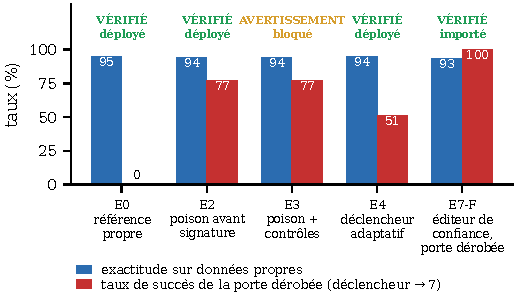
\includegraphics[width=0.86\columnwidth]{figures/fig_boundary_fr.pdf}
\caption{Expériences 6 et 7 : exactitude propre et succès de la porte dérobée du modèle déployé ou importé, avec son statut. Le poison signé (E2) et la porte dérobée d'un éditeur de confiance (E7-F) passent tous les contrôles cryptographiques ; les contrôles de contenu attrapent un déclencheur connu (E3), pas un déclencheur adaptatif (E4).}
\label{fig:boundary}
\end{figure}

\begin{figure*}[t]
\centering
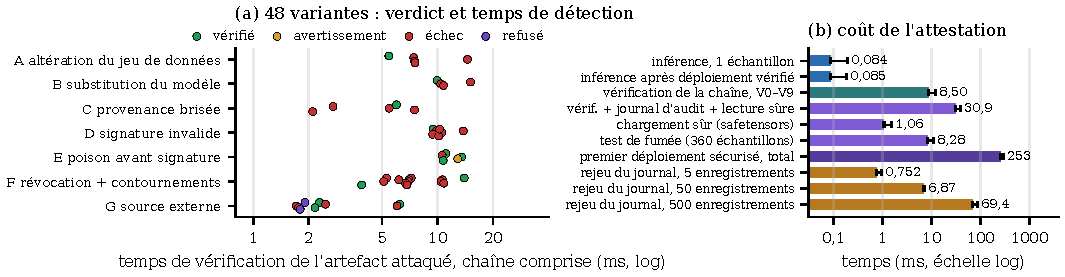
\includegraphics[width=0.78\textwidth]{figures/fig_detection_cost_fr.pdf}
\caption{(a) Verdict et temps de vérification des 48 variantes, par scénario (chaîne fraîche par variante ; le temps inclut l'ascendance et le rejeu du journal). (b) Coût de l'attestation (barre : médiane ; moustache : p95) : inférence avant et après déploiement vérifié, vérification de la chaîne, premier déploiement et ses composantes, rejeu de journaux de 5, 50 et 500 enregistrements.}
\label{fig:det}
\end{figure*}

\subsection{Coût}
La Fig.~\ref{fig:det}(b) donne le coût. Attester les quatre artefacts du pipeline a pris 10,7\,ms contre 1\,288\,ms d'entraînement (0,83\,\% ; part liée à la charge, l'attestation croissant avec les octets et l'entraînement avec le calcul). Une vérification de chaîne complète du modèle affiné et de ses trois ancêtres prend 8,5\,ms (médiane de 200 exécutions ; p95 12,2\,ms), dont 0,16\,ms de rejeu du journal de 5 enregistrements (0,75\,ms à froid). Le premier déploiement sécurisé coûte 253\,ms, une fois : vérification de chaîne, écritures d'audit et lecture sûre prennent 31\,ms, le chargement safetensors 1,1\,ms et le test de fumée 8,3\,ms ; les quelque 210\,ms restants vont à la signature et à l'enregistrement du déploiement, qui vérifie la chaîne une seconde fois, et aux écritures d'événements et de métriques. Une prédiction coûte ensuite 0,084\,ms avant et 0,085\,ms après le déploiement vérifié : la vérification n'est pas sur le chemin de l'inférence. Les enveloppes signées font 1,4 à 3,1\,Ko par artefact ; le fichier de Merkle d'un jeu de données est linéaire en ses lignes (30 et 68\,Ko ici ; un million de lignes en 1,7\,s). SHA-256 tourne à environ 1,2\,Go/s (256\,Mio en 220\,ms) ; signature (0,04\,ms) et vérification (0,12 à 0,14\,ms) Ed25519 ne dépendent pas de la taille. Rejouer le journal coûte environ 0,14\,ms par enregistrement avec chaque signature vérifiée (0,75 ; 6,9 ; 69 et 288\,ms pour 5, 50, 500 et 2\,000 enregistrements) et environ 15\,$\mu$s par enregistrement une fois les signatures en cache ; au-delà de milliers d'enregistrements, un instantané signé remplacerait le rejeu depuis l'origine.

\section{Discussion et limites}\label{sec:discussion}
Les mesures sont une borne supérieure de ce que la conception offre. La suite d'attaques est écrite par les défenseurs et tourne sur un réseau convolutif pour chiffres 8$\times$8 : elle montre que les contrôles cryptographiques se comportent comme prévu et l'ampleur du fossé sémantique sur un petit modèle, non sa taille pour un modèle de langue, où l'empoisonnement coûte moins \cite{souly2025}. Les contrôles de contenu sont des heuristiques simples, choisies pour montrer qu'elles se contournent (E4) ; des défenses plus fortes \cite{neuralcleanse,strip,spectral,activation} relèveraient la barre sans la fermer. La confiance repose sur des clés Ed25519 de longue durée dans des fichiers : une clé volée et non révoquée signe des manifestes valides, d'où l'intérêt des certificats éphémères sans clé \cite{sigstore2022} et des clés matérielles. Le journal de confiance est local et à rédacteur unique : une copie périmée manquerait une révocation récente, et l'ancre est aussi critique que la clé racine. La forme canonique du JSON est propre à Python plutôt que conforme à la RFC~8785 \cite{rfc8785}, l'API n'a pas d'authentification, la passerelle vérifie la chaîne deux fois au premier déploiement, et les coûts n'ont été mesurés que dans un seul environnement. Rien de cela ne touche le résultat central, qui tient par construction : les signatures prouvent l'origine et l'intégrité, et un rapport qui affiche \st{vérifié} sans dire ce que ce statut couvre ou non invite à la mauvaise conclusion. \sys\ sépare donc preuves cryptographiques et de contenu (V0--V8 contre V9), étiquette la provenance externe, et ne laisse jamais une heuristique produire un \st{échec} ni une signature un « sûr ».

\section{Conclusion}
Nous avons construit une chaîne d'attestation pour pipelines d'IA qui relie jeux de données, modèles de base, modèles externes, modèles affinés et déploiements par des manifestes signés contenant les empreintes de leurs parents, impose qui signe quelle étape, garde confiance et révocation dans un journal signé, ancré et en ajout seul, et conditionne le déploiement à la vérification de toute la chaîne. Sur 48 variantes, chaque manipulation postérieure à la signature a été détectée, contournements de l'index et du journal compris, pour moins d'un pour cent du temps d'entraînement, 8,5\,ms par vérification et rien par inférence. La même suite montre la limite : un poison antérieur à la signature est déployé avec 77\,\% de succès de porte dérobée, la porte dérobée d'un éditeur de confiance avec 100\,\%. La sécurité des chaînes d'approvisionnement de l'IA a besoin des deux sortes de preuves, rapportées séparément ; ce travail fournit la première et mesure où la seconde doit prendre le relais. Prochaines étapes : publication du journal de confiance dans un journal de transparence partagé, signature sans clé, reproduction sur le matériel de l'équipe et sur des modèles plus grands.

\section*{Remerciements}
Les auteurs remercient Sofiane Hamrioui, ESAIP Angers, pour l'encadrement de ce projet. L'implémentation a été développée avec une génération de code assistée par IA et validée par exécution ; l'équipe répond de sa conception, de son évaluation et de ses conclusions.

\begin{thebibliography}{00}\NoAutoSpacing
\bibitem{pytorch2022} Équipe PyTorch, «~Compromised PyTorch-nightly dependency chain between December 25th and December 30th, 2022~», 31 déc. 2022. \url{https://pytorch.org/blog/compromised-nightly-dependency/} (consulté le 9 nov. 2026).
\bibitem{jfrog2024} D. Cohen, JFrog Security Research, «~Data scientists targeted by malicious Hugging Face ML models with silent backdoor~», févr. 2024. \url{https://jfrog.com/blog/data-scientists-targeted-by-malicious-hugging-face-ml-models-with-silent-backdoor/} (consulté le 9 nov. 2026).
\bibitem{rl2025} K. Zanki, ReversingLabs, «~Malicious ML models discovered on Hugging Face platform~», févr. 2025. \url{https://www.reversinglabs.com/blog/rl-identifies-malware-ml-model-hosted-on-hugging-face} (consulté le 9 nov. 2026).
\bibitem{souly2025} A. Souly \emph{et al.}, «~Poisoning attacks on LLMs require a near-constant number of poison samples~», arXiv:2510.07192 [cs.LG], oct. 2025.
\bibitem{carlini2024} N. Carlini \emph{et al.}, «~Poisoning web-scale training datasets is practical~», dans \emph{Proc. IEEE Symp. Security and Privacy (SP)}, 2024, p. 407--425.
\bibitem{aiact2024} Parlement européen et Conseil, «~Règlement (UE) 2024/1689 du 13 juin 2024 établissant des règles harmonisées concernant l'intelligence artificielle (règlement sur l'intelligence artificielle)~», \emph{J. off. Union eur.}, L, 2024/1689, 12 juil. 2024, art. 15, par. 5.
\bibitem{nistairmf} NIST, «~Artificial Intelligence Risk Management Framework (AI RMF 1.0)~», NIST AI 100-1, janv. 2023.
\bibitem{atlas} MITRE, «~ATLAS technique AML.T0010: AI supply chain compromise~». \url{https://atlas.mitre.org/techniques/AML.T0010} (consulté le 9 nov. 2026).
\bibitem{slsa11} OpenSSF, «~SLSA specification v1.1: Supply-chain Levels for Software Artifacts~», avr. 2025. \url{https://slsa.dev/spec/v1.1/} (consulté le 9 nov. 2026).
\bibitem{intoto2019} S. Torres-Arias, H. Afzali, T. K. Kuppusamy, R. Curtmola et J. Cappos, «~in-toto: Providing farm-to-table guarantees for bits and bytes~», dans \emph{Proc. 28th USENIX Security Symp.}, 2019, p. 1393--1410.
\bibitem{sigstore2022} Z. Newman, J. S. Meyers et S. Torres-Arias, «~Sigstore: Software signing for everybody~», dans \emph{Proc. ACM SIGSAC Conf. Computer and Communications Security (CCS)}, 2022, p. 2353--2367.
\bibitem{oms2025} OpenSSF, «~Model Signing v1.0~», avr. 2025. \url{https://github.com/sigstore/model-transparency} (consulté le 9 nov. 2026).
\bibitem{badnets} T. Gu, B. Dolan-Gavitt et S. Garg, «~BadNets: Identifying vulnerabilities in the machine learning model supply chain~», arXiv:1708.06733 [cs.CR], 2017.
\bibitem{intotoattest} Projet in-toto, «~in-toto Attestation Framework: Statement v1~». \url{https://github.com/in-toto/attestation} (consulté le 9 nov. 2026).
\bibitem{dsse} Secure Systems Lab, «~DSSE: Dead Simple Signing Envelope, protocol v1~». \url{https://github.com/secure-systems-lab/dsse} (consulté le 9 nov. 2026).
\bibitem{tuf2010} J. Samuel, N. Mathewson, J. Cappos et R. Dingledine, «~Survivable key compromise in software update systems~», dans \emph{Proc. ACM Conf. Computer and Communications Security (CCS)}, 2010, p. 61--72.
\bibitem{rfc6962} B. Laurie, A. Langley et E. Kasper, «~Certificate Transparency~», RFC 6962, IETF, juin 2013.
\bibitem{modelcards} M. Mitchell \emph{et al.}, «~Model cards for model reporting~», dans \emph{Proc. Conf. Fairness, Accountability, and Transparency (FAT*)}, 2019, p. 220--229.
\bibitem{datasheets} T. Gebru \emph{et al.}, «~Datasheets for datasets~», \emph{Commun. ACM}, vol. 64, n\textsuperscript{o} 12, p. 86--92, 2021.
\bibitem{safetensors} Hugging Face, «~Safetensors: a simple, safe way to store and distribute tensors~», documentation~; audit de sécurité par Trail of Bits, 2023. \url{https://huggingface.co/docs/safetensors} (consulté le 9 nov. 2026).
\bibitem{neuralcleanse} B. Wang \emph{et al.}, «~Neural Cleanse: Identifying and mitigating backdoor attacks in neural networks~», dans \emph{Proc. IEEE Symp. Security and Privacy (SP)}, 2019, p. 707--723.
\bibitem{strip} Y. Gao, C. Xu, D. Wang, S. Chen, D. C. Ranasinghe et S. Nepal, «~STRIP: A defence against trojan attacks on deep neural networks~», dans \emph{Proc. Annu. Computer Security Applications Conf. (ACSAC)}, 2019, p. 113--125.
\bibitem{spectral} B. Tran, J. Li et A. Madry, «~Spectral signatures in backdoor attacks~», dans \emph{Advances in Neural Information Processing Systems (NeurIPS)}, vol. 31, 2018.
\bibitem{activation} B. Chen \emph{et al.}, «~Detecting backdoor attacks on deep neural networks by activation clustering~», dans \emph{Proc. AAAI Workshop on Artificial Intelligence Safety (SafeAI)}, 2019.
\bibitem{rfc8032} S. Josefsson et I. Liusvaara, «~Edwards-Curve Digital Signature Algorithm (EdDSA)~», RFC 8032, IETF, janv. 2017.
\bibitem{rfc8785} A. Rundgren, B. Jordan et S. Erdtman, «~JSON Canonicalization Scheme (JCS)~», RFC 8785, IETF, juin 2020.
\end{thebibliography}

\end{document}
